\documentclass{article}
\usepackage{graphicx}
\usepackage[french]{babel}
\usepackage{multicol}
\usepackage{geometry}
\usepackage{titling}
\usepackage[utf8]{inputenc}
\usepackage{natbib}
\usepackage[style=authoryear,backend=biber]{biblatex}
\usepackage{hyperref}

\addbibresource{name.bib}




\geometry{
    a4paper,
    total={170mm,257mm},
    left=20mm,
    top=30mm,
}



\title{
    
\includegraphics[width=1\textwidth]{photo/UCLouvain_Charleroi.png} \\
    \vspace{1.5cm}
    {\Huge \textbf{Rapport personnelle projet vis}} \\
    \vspace{1.5cm}
}

\author{
    \textbf{Moussaoui Noah} \\
    Université catholique de Louvain-la-Neuve \\
    Campus de Charleroi, EPL en SINC \\
    Délégué et ambassadeur \\
    \texttt{Noah.moussaoui@student.uclouvain.be}
}

\date{
    \vspace{1.5cm}
    Durée de recherche : Septembre - Novembre \\
     \vspace{1.5cm}
    
\includegraphics[width=0.5\textwidth]{photo/EPL.png}
}

\begin{document}

\maketitle
\newpage
\section{Introduction}
Dans ce projet, nous avons travaillé sur une application mobile dont l'objectif est de permettre 
aux utilisateurs de rencontrer des requins, mais sans adopter le format traditionnel des applications
de rencontres. Il s'agit plutôt d'un réseau social où les utilisateurs peuvent se retrouver pour 
"chasser" des humains, consulter des publications, découvrir des propositions d’événements, 
et regarder des stories.\\\\

Ensemble, nous nous appuyons sur les données d’un fichier CSV contenant des informations 
sur différentes attaques de requins dans le monde, données qui alimenteront bien sûr notre application.


\section{Personas}
Voici différents Personas qui sont des potentile client de notre application \\

Mon persona:\\

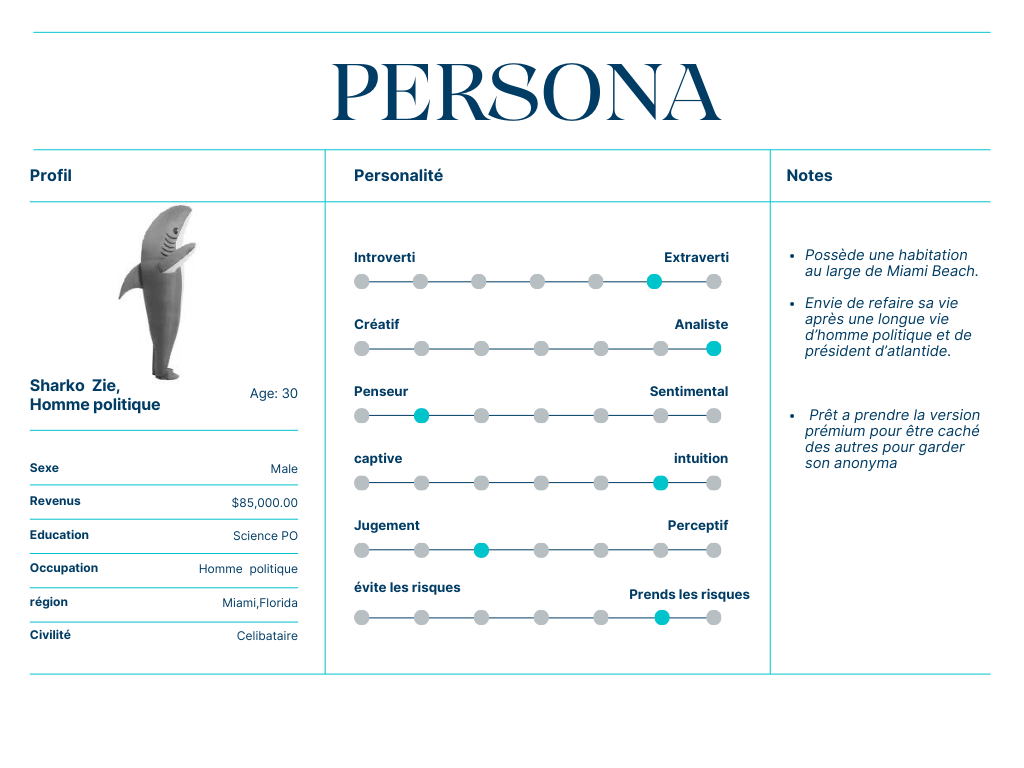
\includegraphics[width=1\textwidth]{photo/Personna_Sharkozie.png}\\

Voici mon persona Sharko Zie \\

Il serait interessé par l'applis et surtout de son mode prémium qui lui permet de garder l'anonymat
car oui Sarko ne veut pas qu'on voit qu'un ancient président recherche des amis pour chasser mais aussi
pour son VPN qui permet à Mr. Sharko Zie de changer sa localisation pour trouver des amis pour chasser
quand il part en vacance . \\

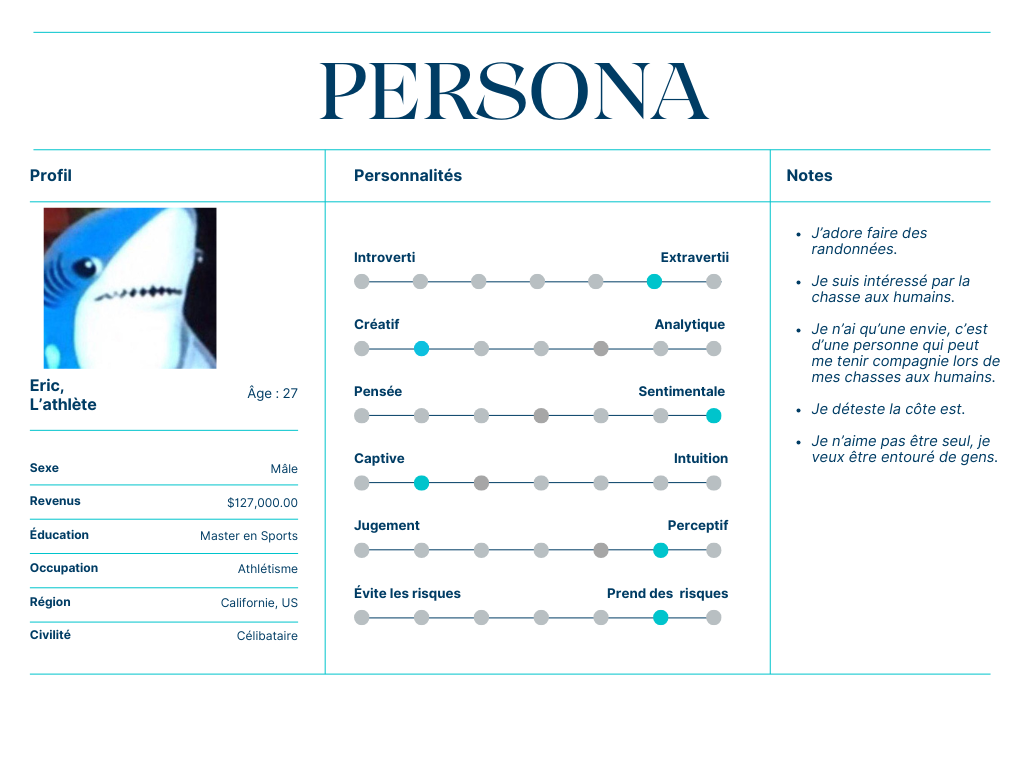
\includegraphics[width=1\textwidth]{photo/Personna_Kaan.png}\\

Voici Eric L'athlète\\

Eric est quelqu'un de très social dans la vie il aime avoir beaucoup d'amis et partager sa vie il serait 
un très grand client des stories et des posts sur le fil d'actualité .  Malheuresement l'applis à des ajouts 
d'amis est limité par jours mais la version prémium peut changer cela et mettre l'ajout d'amis ilimité . 
Eric n'aime pas la cote est ils seraient donc aussi client du prémium pour bloquer les gens de la cote est 
pas les voirs sur son fil 







\section{Base-fidélité}


\section{conclusion}


\end{document}
